\chapter{INTRODUCTION}
Streaming data is exploding. 
Applications such as Facebook and Twitter are constantly streaming the data that can be consumed by a wide range of streaming applications.
A key task for almost all stream processing systems, from moment to moment, is to figure out which data to remember and which to forget, in a computationally efficient manner. 
This dissertation approaches this task with the concept of ``data important''.
The core contributions include an extensible conceptual model called \textbf{semantic importance}, as well as a set of infrastructure for its general applications in stream reasoning contexts, as shown in Figure \ref{fig:1-tv}.

\begin{figure}[!htbp]
	\centering
    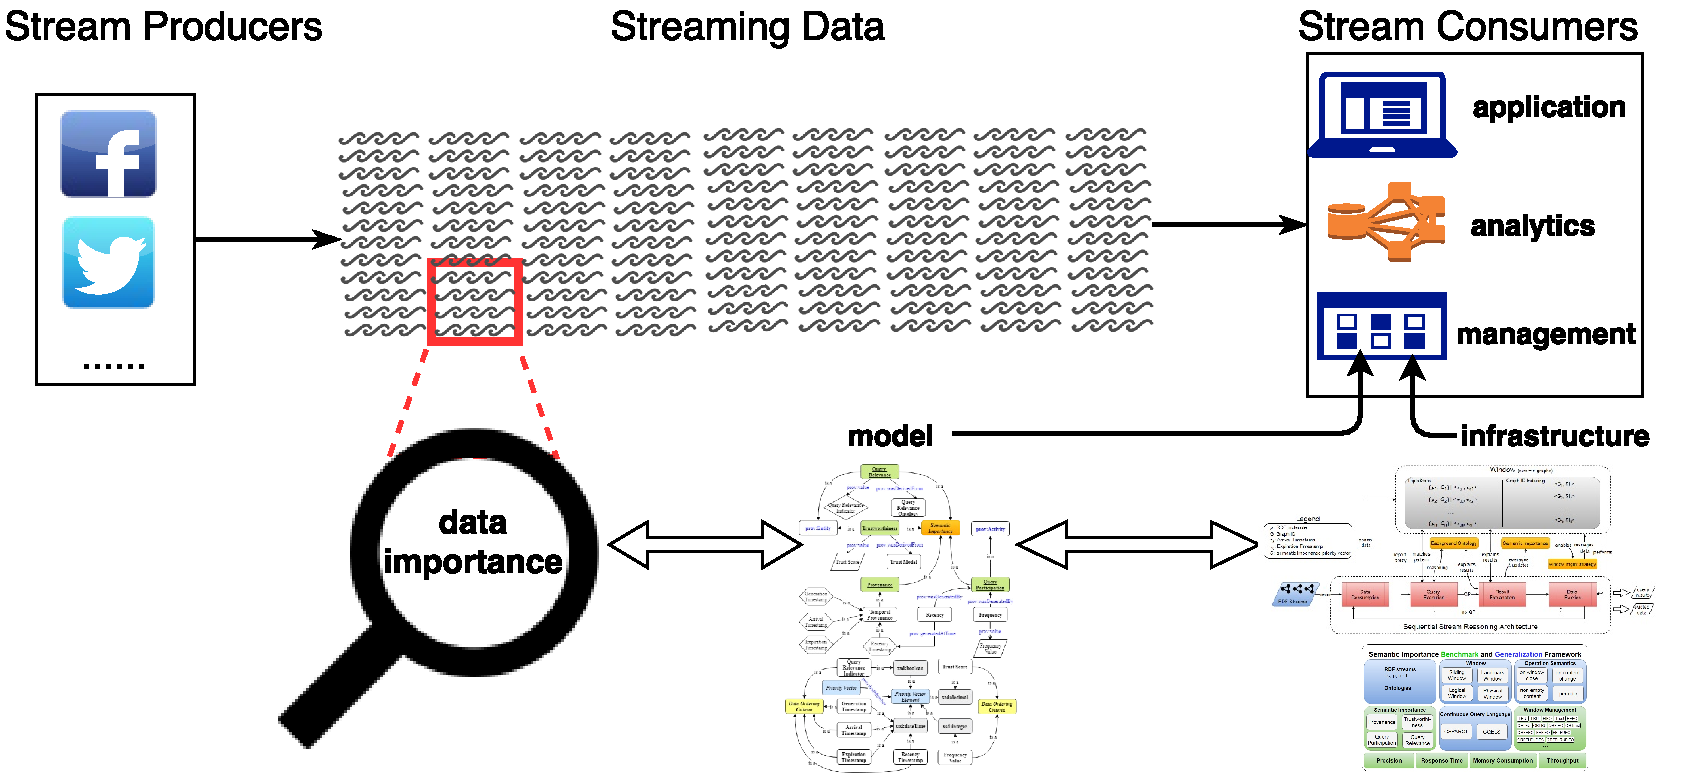
\includegraphics[width=5in]{img/1-tv.pdf}
    \caption{\textbf{Dissertation Vision}}
    \label{fig:1-tv}
\end{figure}

Streaming data is boundless, enormous, and frequently updated \cite{rodriguez2009semantic}.
It usually has intrinsic orders. 
For example, when a sequence of streaming data items arrive at the system, they are stamped with arrival timestamps.
This arrival ordering is only scratching the surface, because there are many other data orderings. 
Data can be ordered by when it is expired, where it comes from, how much it can be trusted, how precise it is, how relevant it is to the query, etc \cite{della2013order}. 

Stream reasoning, defined as ``logical reasoning in real time on gigantic and inevitably noisy data streams in order to support decision process of extremely large number of concurrent users'' \cite{barbieri2010stream}, is a newly identified research area that aims to bridge semantic reasoning with stream processing, so as to extract hidden information out of the streams.
Stream reasoning processes RDF streams \cite{barbieri2010querying}, defined as ``an infinite ordered sequence of data items'' \cite{srtutorial}, that model data streams by extending RDF.
The data items in RDF streams can be either triples or graphs, annotated by time-point timestamps or time-interval timestamps.

Stream reasoning has two key notions \cite{barbieri2010stream}, the sliding window \cite{arasu2003stream} and continuous processing \cite{babu2001continuous}.
A sliding window, or more generally a window, is a finite subset of the data stream, and manages the data.
Continuous processing repeatedly evaluates the data in the window as the window proceeds. 
The sliding window has two parameters, a size and a step \cite{stuckenschmidt2010towards}.
The size indicates how much data an active window can hold.
The step describes how far a window can move at one time.
According to the defined sliding window semantics \cite{botan2010secret}, a sliding window's size and step should be both fixed over the same stream. 

Windows have different types \cite{barbieri2010querying}:
a logical or temporal window has its step and size defined in the time domain; 
a physical or tuple window has a tuple-based step and size.
Windows can also be categorized based on the relationship between the size ($l$) and step ($d$):
if $d < l$, it is a sliding window;
if $d = l$, it is a tumbling window;
if $d > l$, it is a sampling window \cite{calbimonte2010enabling}. 
The behavior of a window is modeled by window operational semantics \cite{botan2010secret} \cite{dell2013correctness}. 
It includes four aspects: scope, content, report and tick. 
Scope not only determines the boundary of an active window, but also affects the starting time ($t_{0}$) of the continuous processing.
Content describes the subset of the data stream that is currently in an active window.
Report defines the condition to fire the query.
Common policies include ``on content change'', ``on window full'', ``non-empty content'' and ``periodic''.
Tick defines how and when to react to the input, which can be either tuple-driven or time-driven.  
%
\section{The Silent Temporal Assumption}

\begin{figure}[!htbp]
	\centering
    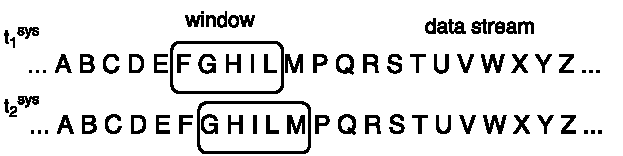
\includegraphics[width=5in]{img/1-sta.pdf}
    \caption{\textbf{The Silent Temporal Assumption}}
    \label{fig:1-sta}
\end{figure}

Figure \ref{fig:1-sta} shows a data stream being processed by two windows at $t^{sys}_1$ and $t^{sys}_2$ time respectively. 
Data is processed under a popular window management strategy called first in first out (FIFO), such that the window will have to evict the oldest data item A in order to consume the latest data item B at $t^{sys}_{2}$.
FIFO is based on the \textbf{silent temporal assumption} that ``older information becomes irrelevant at some point'' \cite{barbieri2010stream} \cite{stuckenschmidt2010towards}.
A lot of stream reasoning work is based on this assumption.
For example, 
``... new items are often more accurate and relevant than older items ...'' \cite{golab2003processing};
``... recent items are typically more relevant than older ones ...'' \cite{barbieri2010deductive}.

FIFO is computationally efficient, but ultimately problematic depending on the window size and streaming data characteristics. 
This dissertation will show the problems related to the silent temporal assumption, as well as the approaches to solve the problems by loosening this assumption. 
%
\section{A Running Example}
In general, not all of the data items in streams can be used to answer the query \cite{mileo2013streamrule}.
There are situations where a single data item contains sufficient information (Situation 1), or multiple data items are required (Situation 2), so as to provide query answers. 
For the sake of convenience, this dissertation uses a term called \textbf{necessary data item} to refer to the data items that contain necessary information for question answering. 

The FIFO window management strategy based on the silent temporal assumption can work well in Situation 1. 
For Situation 2, the answer will only be returned when all of the necessary data items exist in the window at one time-point. 
However, the distance among necessary data items can be arbitrarily apart, and if this distance is longer than the window size, false answers will be generated. 
In order to illustrate this problem, this dissertation uses a running example of real-life soccer offside offence detection.

\begin{figure}[!htbp]
	\centering
	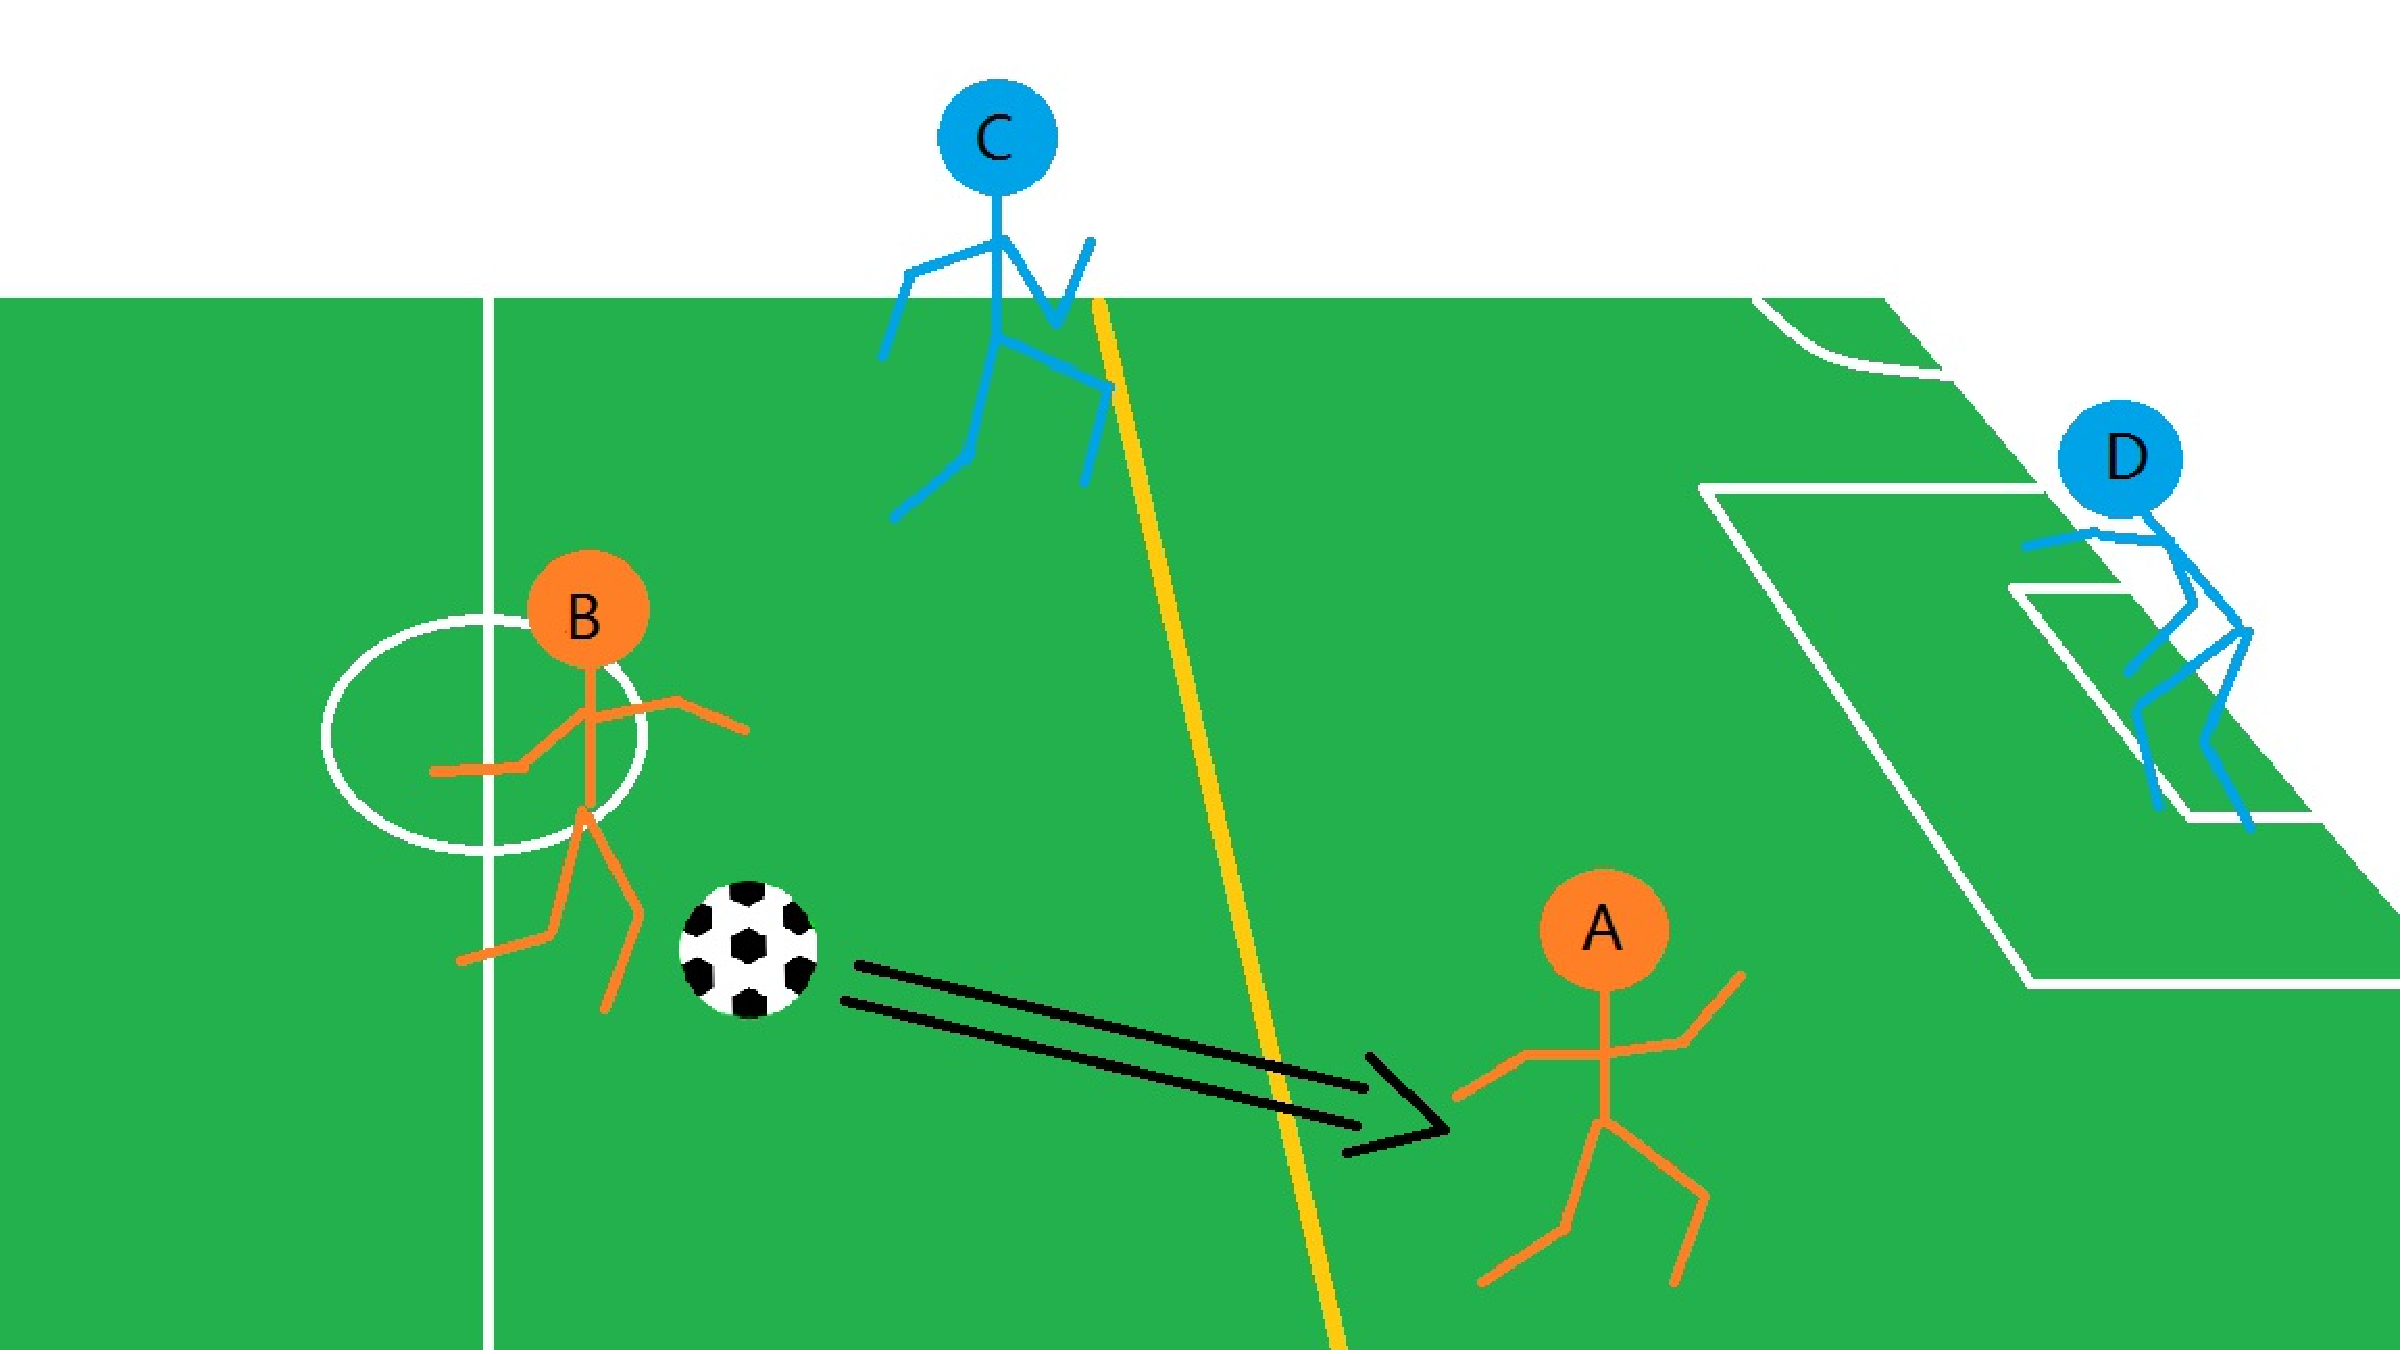
\includegraphics[width=5in]{img/1-soe.pdf}
	\caption{\textbf{A Soccer Offside Example}}
	\label{fig:1-soe} 
\end{figure}

Soccer offside offence is a common offence, which easily decides the direction where the game goes, thus can be very controversial sometimes.
F\'ed\'eration Internationale de Football Association (FIFA) defines soccer offside offence in a comprehensive way \cite{federation2016laws}. 
In this dissertation, a simplified definition will be used: 
a soccer offside offence is committed if an attacker who is at an offside position involves in an active play. 
So there are three atomic data items needed in order to determine an offside offence:
an attacker who is a member of a team that controls the ball;
this attacker is at an offside position that is nearer to the opponent's goal line than both the second last defender and the ball;
and this attacker involves in an active play, meaning that he/she either touches the ball or challenges an opponent. 
Figure \ref{fig:1-soe} shows a soccer offside offence example, where Player A and B are attacking.
Player A is at an offside position indicated by the yellow line. 
The moment that Player A becomes the first person to touch the ball passed from B is when an offside offence is committed.

Reasons to use this running example are two-folds.
First, situations in a soccer game can change all the time, thus a soccer offside offence can happen anytime in a very fast period. 
Second, the three atomic data items to determine a soccer offside offence will not arrive at the same time. 
This is because time will elapse as the ball is passed from Player B to Player A, and some other data will be generated during that time, such as players' positional data.

\begin{table}[!htbp]
	\centering
	\caption{\textbf{Soccer Streaming Data Items}}
	\label{tab:icons}
	\begin{tabular}{|c||c|c|c|} \hline
		icon & annotation & example & data sample \\ \hhline{|=#=|=|=|}
    	$\times$ & position & \makecell{$\times_{A}$ \\ $\times^{\circ}_{A}$} & \makecell{:PlayerA :hasPosition :PositionA \\ :PlayerA :hasPosition :OffsideOffencePosition} \\ \hline 
		$\largecircle$ & \makecell{active play \\involvement} & $\largecircle_{A}$ & :PlayerA a :BallLastToucher \\ \hline
		$\largetriangleup$ & attacker & $\largetriangleup_{A}$ & :PlayerA a :Attacker \\ \hline
		$\largesquare$ & defender & $\largesquare_{A}$ & :PlayerA a :Defender \\ \hline
	\end{tabular}
\end{table}

The data stream used for the running example throughout this dissertation contains four different types of data items in Table \ref{tab:icons}.
$\times$ indicates a player's positional data;
$\times^{\circ}$ denotes the offside position of a player; 
$\largetriangleup$ refers to an attacker;
$\largesquare$ describes a defender;
$\largecircle$ represents that some player involves in an active play, such as touching the ball, challenging an opponent, etc.

Together with these denotations, and the logic and-operator ($\wedge$), that Player A commits an offside offence can be expressed as
$\largetriangleup_{A} \wedge \times^{\circ}_{A} \wedge \largecircle_{A}$. 
Players on the field move from time to time, which will make offensive transitions happen at any moment.
Any player can involve in an active play. 
Thus these four kinds of the data items can form a data stream that reflects the situations on the field.
This example also assumes that a stream reasoning application consumes this data stream and constantly looks for players who commit offside offences. 
%
\section{Early Eviction}

\begin{figure}[!htbp]
	\centering
	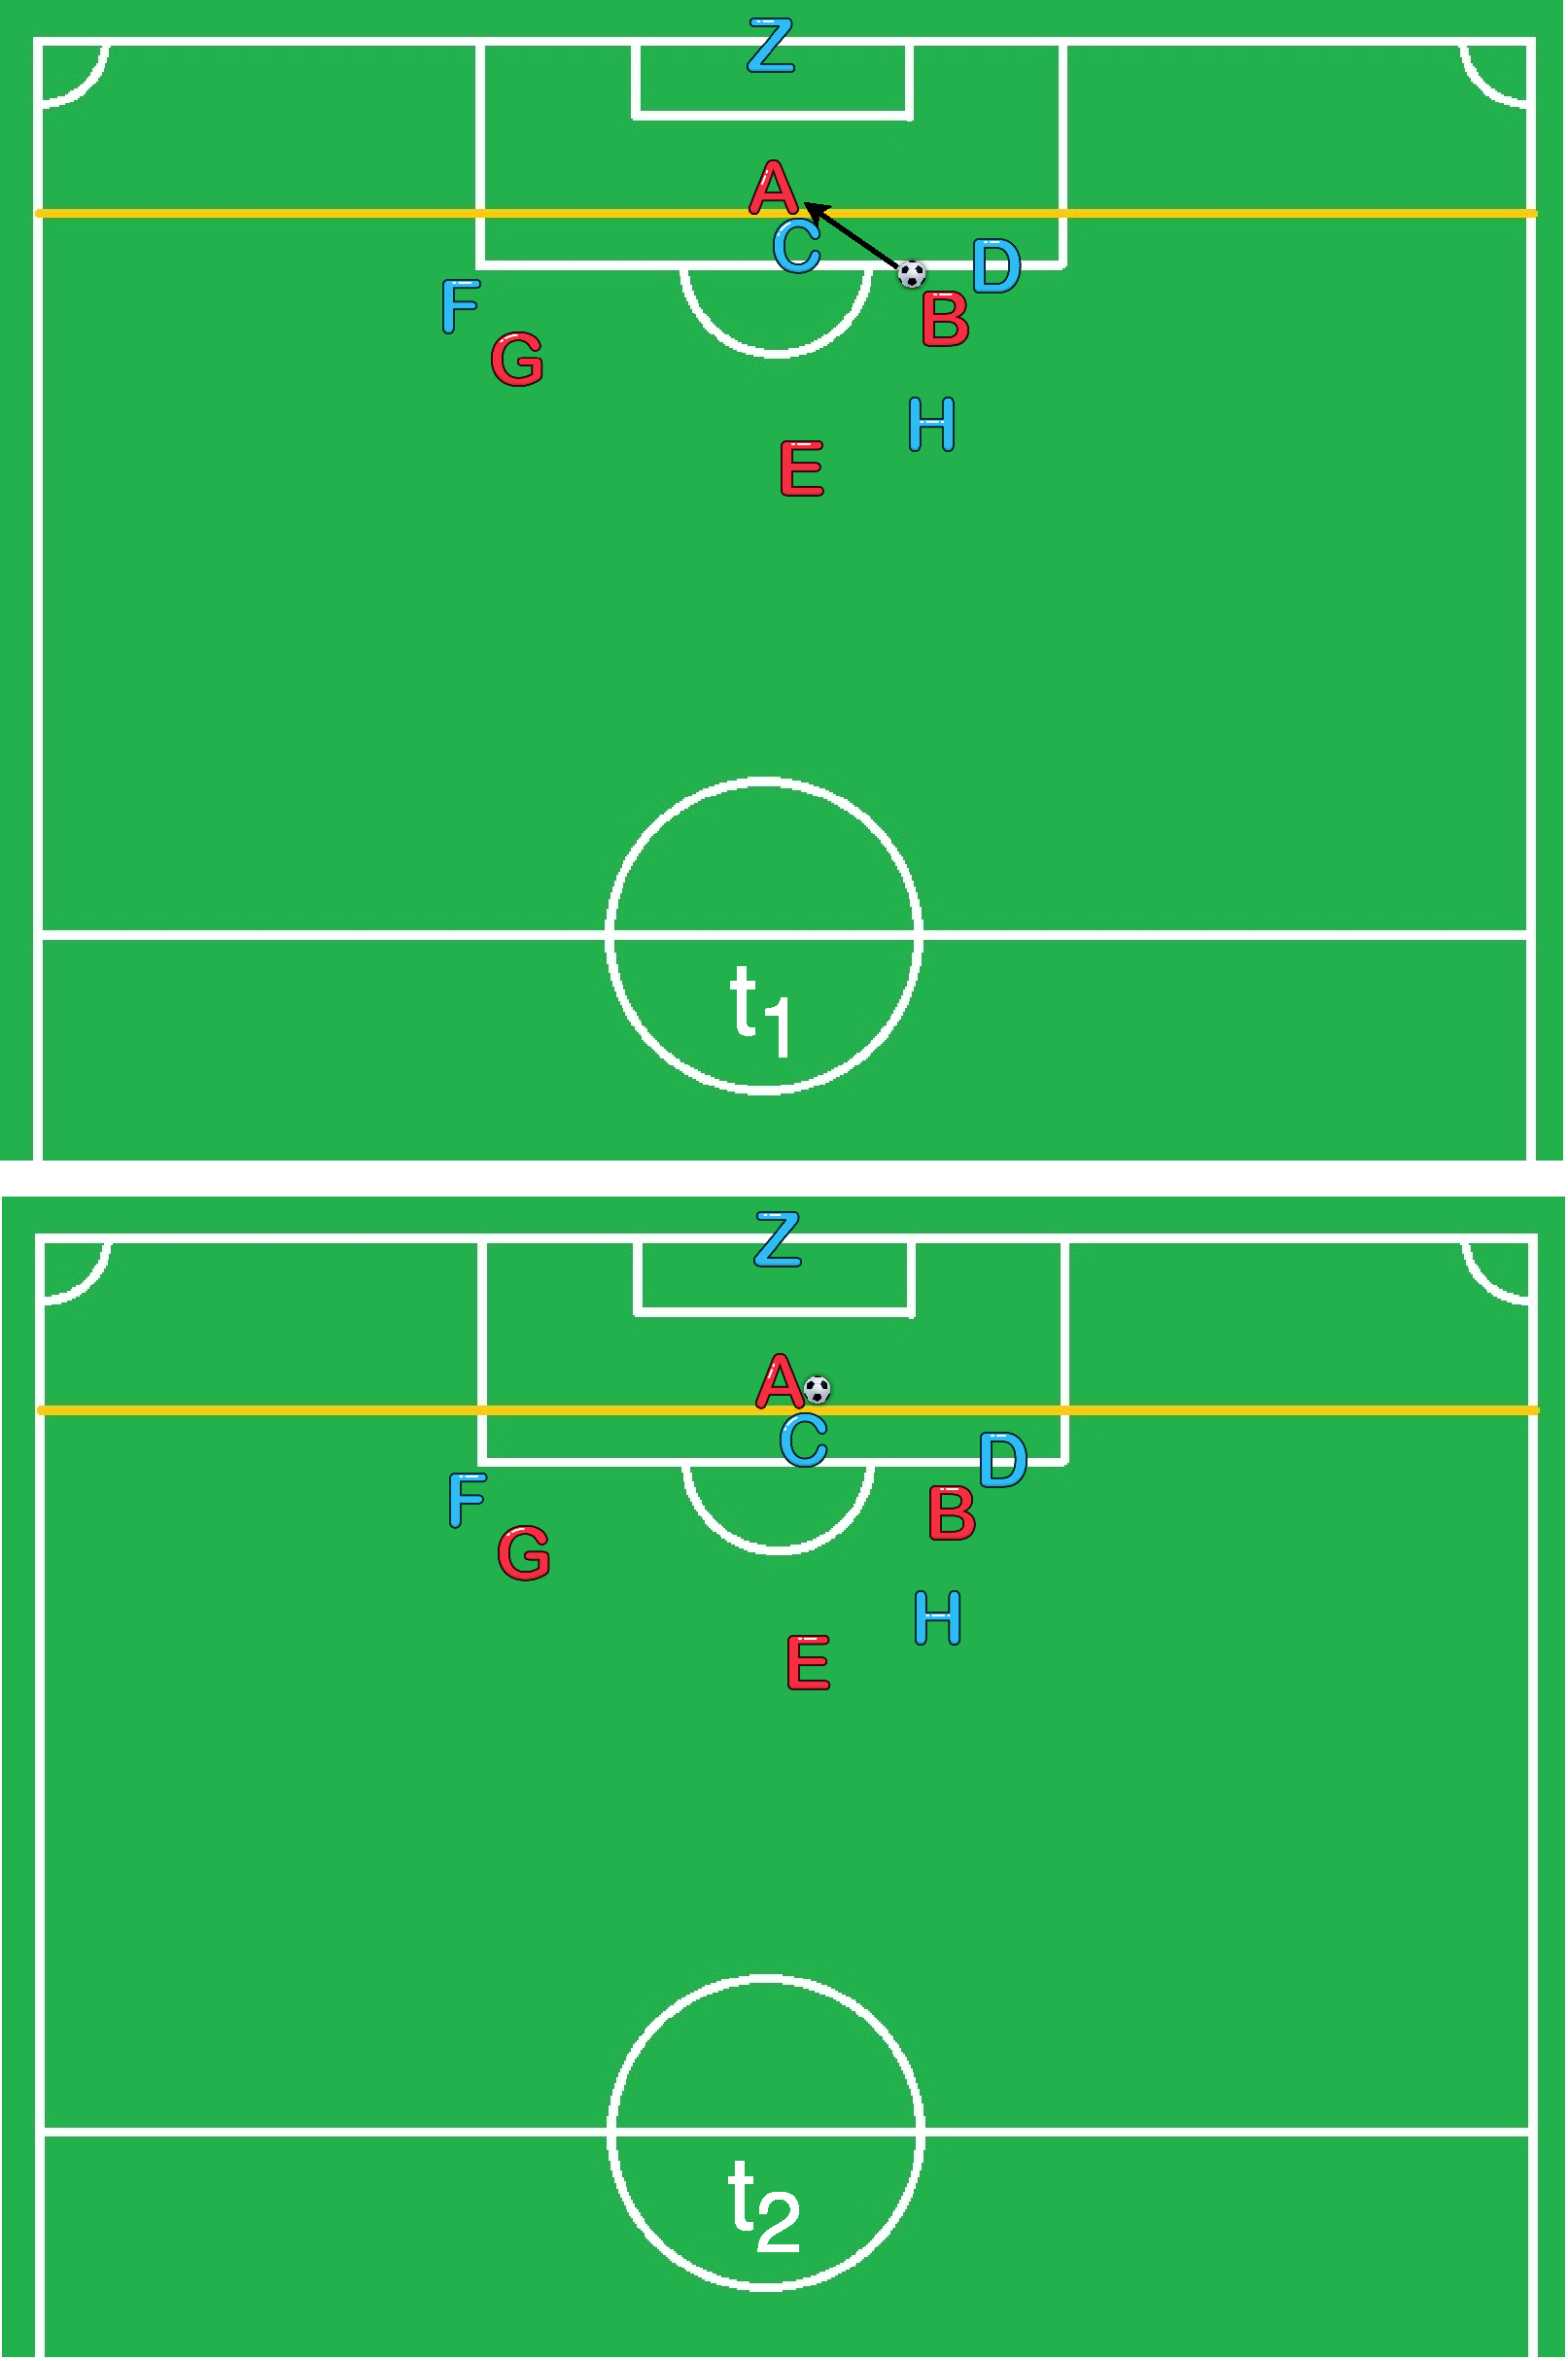
\includegraphics[width=5in]{img/1-seeh.pdf}
	\caption{\textbf{Soccer Offside Early Eviction}}
	\label{fig:1-seeh} 
\end{figure}

Consider the situation in Figure \ref{fig:1-seeh}:
at $t_{1}$ time, red team is attacking.
Player B is passing the ball to Player A who is at an offside position indicated by the yellow line. 
At $t_{2}$ time, Player A is the first one to get the ball and about to take a shot.
At this moment, the linesman flags to notify the referee that Player A commits an offside offence.\footnote{Conventionally, a linesman usually flags if he/she thinks Player A will be the first one to touch the ball so as to help save some stamina.}

\begin{figure}[!htbp]
	\centering
	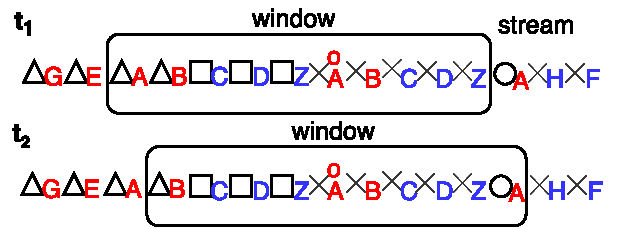
\includegraphics[width=5in]{img/1-seew.pdf}
	\caption{\textbf{Early Eviction in Sliding Window with FIFO}}
	\label{fig:1-seew} 
\end{figure}

Figure \ref{fig:1-seew} shows what is happening in the window. 
At $t_{1}$, $\largetriangleup_{A}$ and $\times^{\circ}_{A}$ are both in the window. 
$\largecircle_{A}$ is about to enter the window. 
However, in order to consume $\largecircle_{A}$, $\largetriangleup_{A}$ has to be evicted because of the silent temporal assumption. 
Thus at $t_{2}$, only $\times^{\circ}_{A}$ and $\largecircle_{A}$ exist in the window. 
In either time-point, there is no way to have all three of the necessary data items in the window, causing a false-negative answer. 
Namely, there should be an offside offence but the system fails to detect it. 
This problem is called \textbf{early eviction}: necessary data items are evicted too early before they can be used to answer queries. 

There is a naive solution to the early eviction problem: 
to increase the window size such that it can hold $\largetriangleup_{A}$, $\times^{\circ}_{A}$, and $\largecircle_{A}$ in the same active window.
Nonetheless, increasing the window size will possibly result in having more data within one window, which can drain more system memory and computation resources. 
Increasing window size based on the exact distance among all necessary data items is also not feasible, as in general data items can be arbitrarily apart, and one cannot foretell these distances.
%
\section{Early Expiration}

\begin{figure}[!htbp]
	\centering
	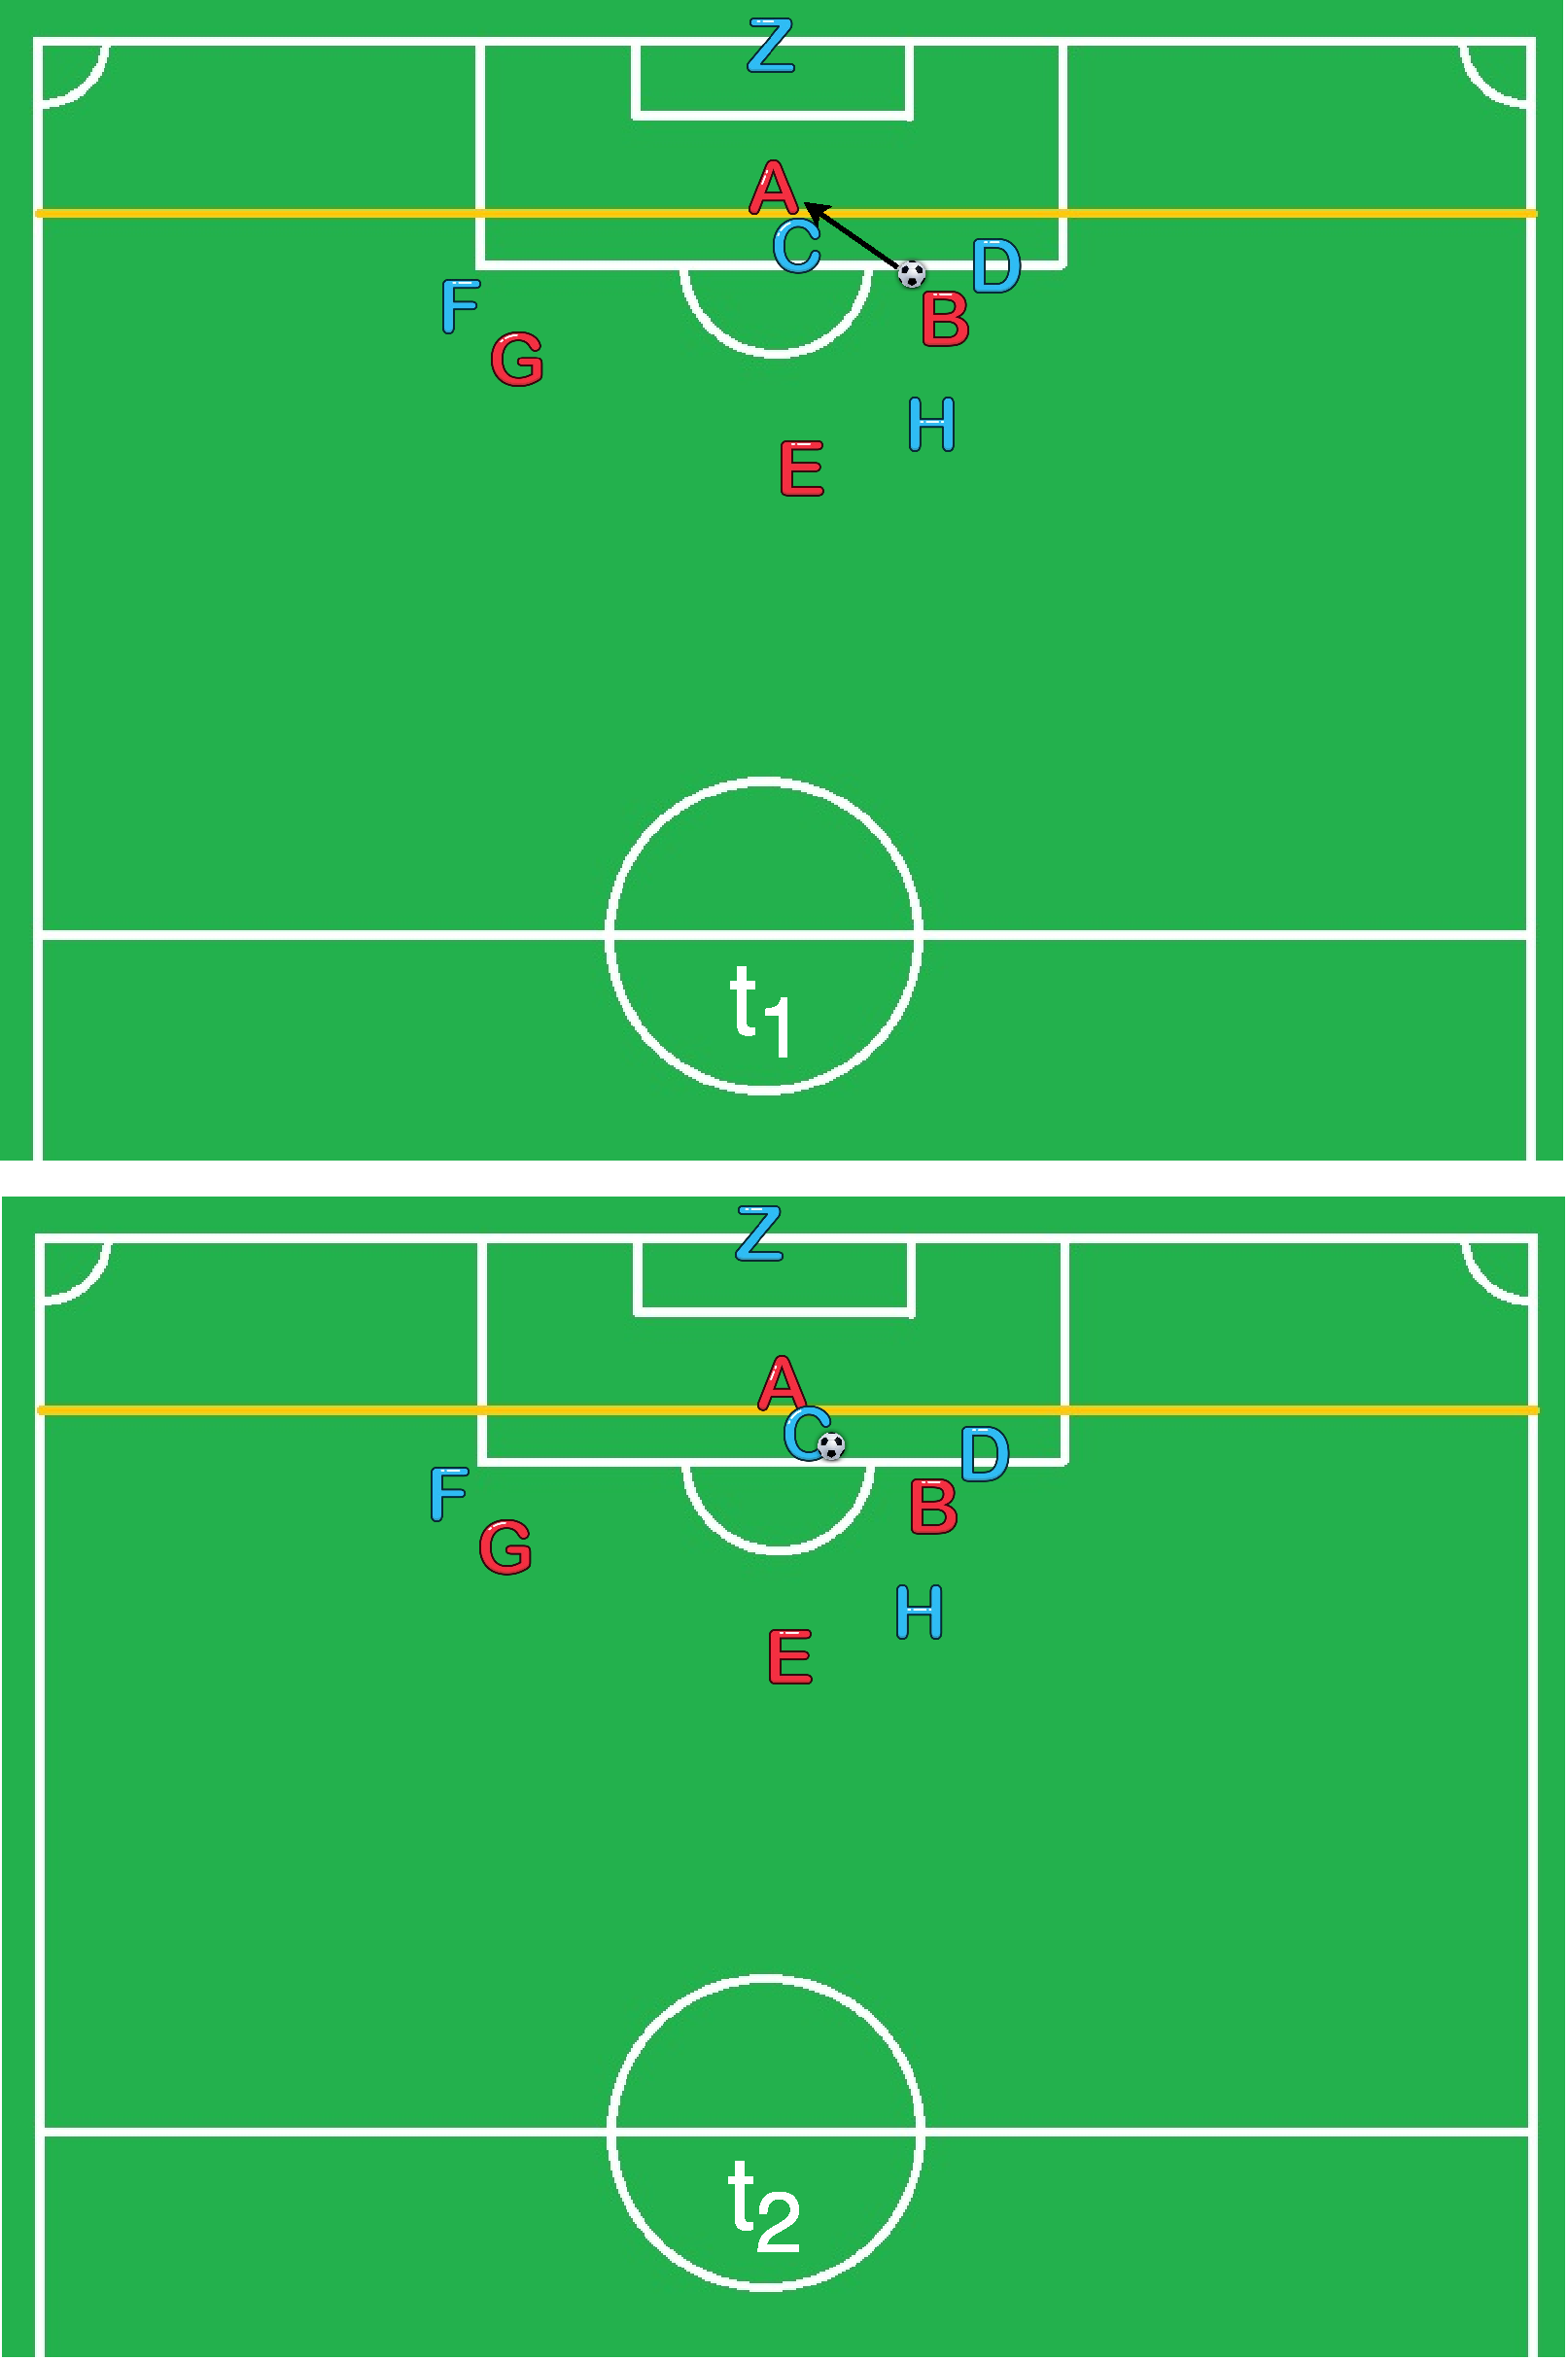
\includegraphics[width=5in]{img/1-seex.pdf}
	\caption{\textbf{Soccer Offside Early Expiration}}
	\label{fig:1-seex} 
\end{figure}

Figure \ref{fig:1-seex} shows another possible situation during a soccer game. 
Again at $t_{1}$, red team is attacking, and Player B is passing the ball to Player A who is at the offside position.
During $t_{1}$ to $t_{2}$, what happens is that Player C successfully steals the ball.
Then Player A immediately challenges Player C in order to grab the ball back. 
At the moment when Player C steals the ball, there is an offensive transition going on.
The blue team is now controlling the ball, thus the red team becomes defensive. 
According to our simplified definition of soccer offside offence, a defender cannot commit an offside offence. 
Thus, the linesman doesn't take any action and let the match continue. 

\begin{figure}[!htbp]
	\centering
	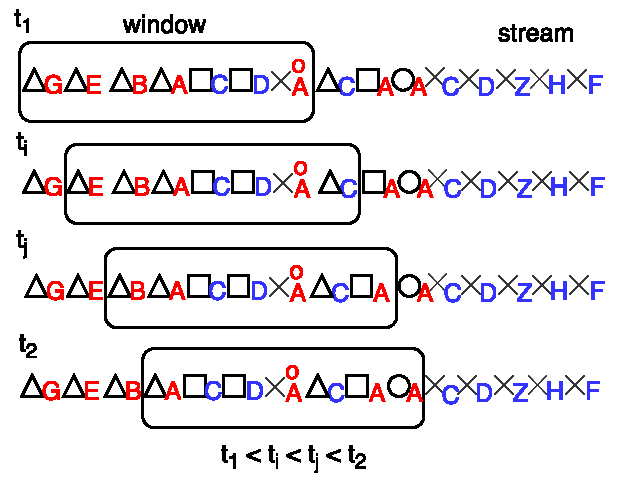
\includegraphics[width=5in]{img/1-seexw.pdf}
	\caption{\textbf{Early Expiration in Sliding Window with FIFO}}
	\label{fig:1-seexw} 
\end{figure}

Figure \ref{fig:1-seexw} shows how sliding window processes the soccer streaming data from Figure \ref{fig:1-seex}. 
As the sliding window moves, $\largetriangleup_{G}$ and $\largetriangleup_{E}$ are successively evicted to make room for $\largetriangleup_{C}$ and $\largesquare_{A}$.
At $t_{i}$, there is already a contradictory: to the window, Player C is both a defender and attacker. 
Although $\largetriangleup_{C}$ and $\largesquare_{C}$ carry different arrival or generation timestamps, these timestamps are only annotations.
For stream reasoning engines such as C-SPARQL \cite{barbieri2010execution}, the continuous query will be parsed into a SPARQL query that is totally blind about the timestamps. 
At $t_{j}$, there is a same contradictory for Player A who is both a defender and an attacker. 
As time reaches $t_{2}$, $\largecircle_{A}$ arrives. 
So all the necessary data items, $\largetriangleup_{A}$, $\times^{\circ}_{A}$, and $\largecircle_{A}$ are in the window, resulting a false-positive answer, i.e. there should not be an offside offence but the system reports positively. 
As a matter of fact, $\largetriangleup_{A}$ should be expired as $\largesquare_{A}$ arrives.
Because there is a transition already happened, the role of Player A is changed from attacker to defender. 
However, due to the silent temporal assumption, the FIFO strategy will not evict $\largetriangleup_{A}$ until after $t_{2}$.
This problem is called \textbf{early expiration}: the data item expires within the window, potentially causing inconsistency or leading to a wrong query answer depending on whether this data item is necessary to answer the query. 
%
\section{Research Hypotheses}
This dissertation is built upon the research hypothesis (RH) that \textit{semantically driven data orderings can effectively capture the data importance. By leveraging data importance modeled from various streaming data orderings, a window in the stream reasoning system can manage data in a smart and flexible way, by which the system precision, response time, memory consumption and throughput can be improved.}
This hypothesis can be represented as a diagram shown in Figure \ref{fig:1-rh}.
Specifically, this hypothesis can be decomposed into following four sub-hypotheses:

\begin{figure}[!htbp]
	\centering
	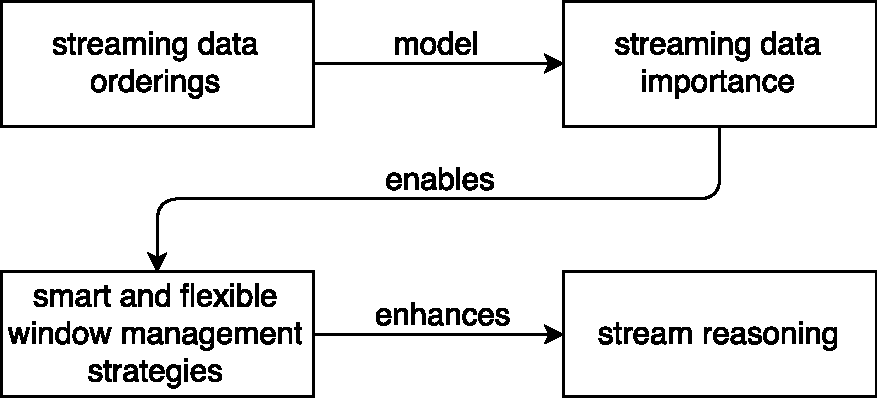
\includegraphics[width=5in]{img/1-rh.pdf}
	\caption{\textbf{Research Hypothesis}}
	\label{fig:1-rh} 
\end{figure}

\textbf{RH1:} \textit{data orderings can model data importance.}
Semantic importance is stated by observing the fact that streaming data usually has intrinsic orderings \cite{della2013order}. 
This not only includes temporal orderings such as arrival/expiration timestamps, but also precision ordering, trust ordering, geo-location ordering, relevance ordering, etc. 
This dissertation hypothesizes that all of these data orderings can be leveraged to model the data importance. 
For example, a data item can be important if it arrives later, or has a bigger trust score, or both. 

\textbf{RH2:} \textit{data importance can enable window management strategies.}
The model of data importance can be used as the window management strategies, which control how window consume, manipulate, query and evict the data.
FIFO is a common strategy under the silent temporal assumption. 
A semantic importance enabled window management strategy possesses the ability to discriminate the data based on its importance. 
Consider if the data itself carries expiration timestamps, the window should pay attention to the data expiration within the window to guarantee valid results.
In this setting, ``not expired'' should be seen as more important. 
An expiration-priority window consumes the most recent data, then evicts all the expired data, then executes the query on it. 
It should also take care of the data expiration during the query execution process. 

\textbf{RH3:} \textit{window management strategies can improve stream reasoning system performance.}
Stream reasoning systems are born with the time constraints, which hinders real-time and correct outputs.
A smaller-sized window holds less data to process, and possibly faster response time, but can potentially provide worse results due to being incapable to hold enough data, especially under the FIFO strategy.
However, if the window can distinguish the right data that can contribute to the query results according to the data importance, the window size can be set to only hold that amount of necessary data. 
In this way, less but enough data for correct results needs to be stored, less computations need to be executed, and more response time is saved, thus the system is able to process more data items within a unit time. 

\textbf{RH4:} \textit{different window management strategies can produce different results.}
Window management strategies are different, which causes the data in the window to be different, even for the same stream. 
The query will be executed on this data, thus the results will be different. 
This hypothesis emphasizes the suitability between the use case requirements and the window management strategies. 
It is critical to deploy suitable strategies in different use cases to maximize the benefits.
%
\section{Research Goal}

\begin{figure}[!htbp]
	\centering
    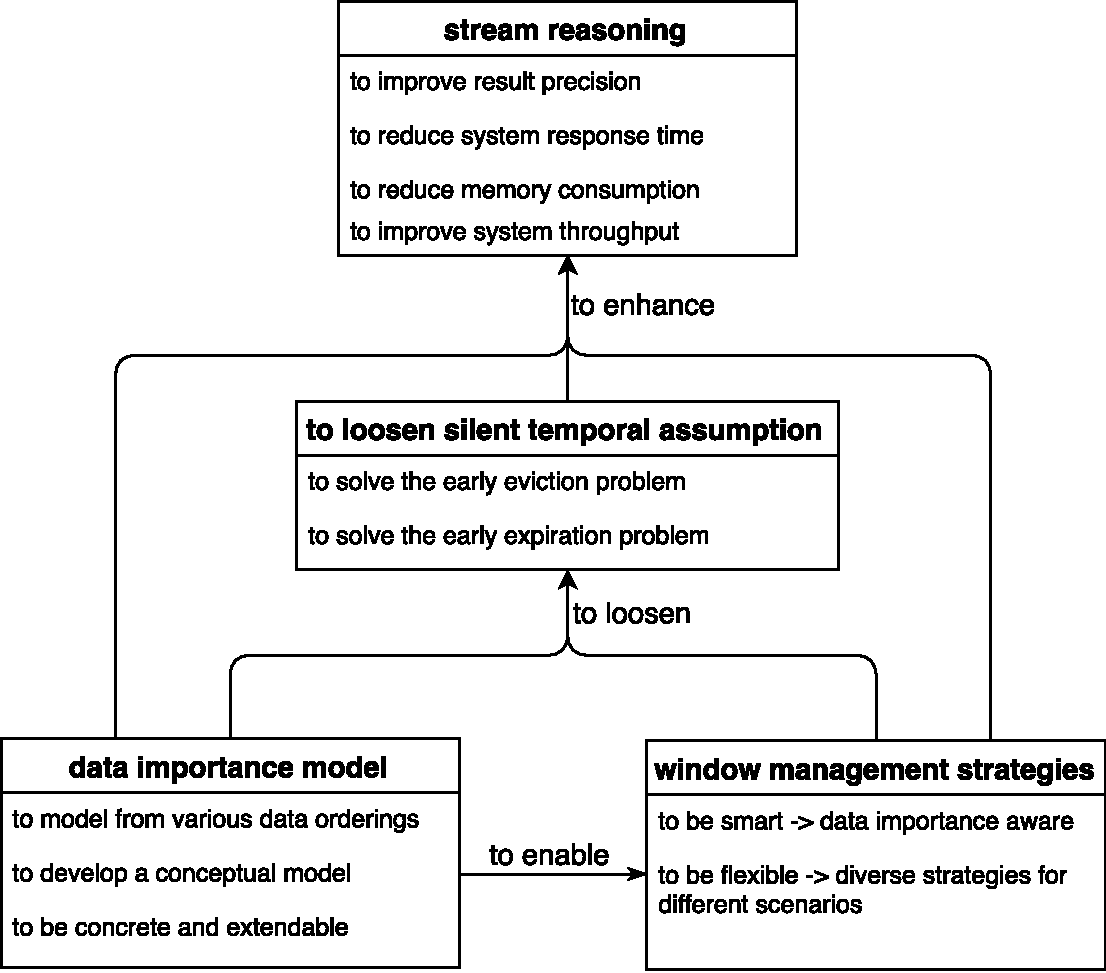
\includegraphics[width=5in]{img/1-rg.pdf}
    \caption{\textbf{Research Goal}}
    \label{fig:1-rg}
\end{figure}

This dissertation aims to achieve the goal in Figure \ref{fig:1-rg}.
This dissertation targets to enhance stream reasoning by loosening the silent assumption via explicitly modeling the importance of the streaming data to the query at hand.
In order to do so, the dissertation will first propose a data importance model developed from various streaming data orderings. 
With this data importance model, smarter and more flexible window management strategies will be enabled. 
The silent temporal assumption can then be loosened by both the model and strategies.
Together with the loosened silent temporal assumption, the data importance model and window management strategies, stream reasoning can be enhanced. 

Specifically, this work will enhance stream reasoning from four perspectives: to improve system precision, to reduce response time, to reduce memory consumption, and to improve system throughput. 
``By loosening the silent assumption'' refers to solving the early eviction and early expiration problems. 
In order to explicitly model the streaming data importance, this dissertation proposes a concrete and expendable semantic conceptual model of data importance and enables smart and flexible window management. 
%
\section{Research Questions}

\begin{figure}[!htbp]
	\centering
	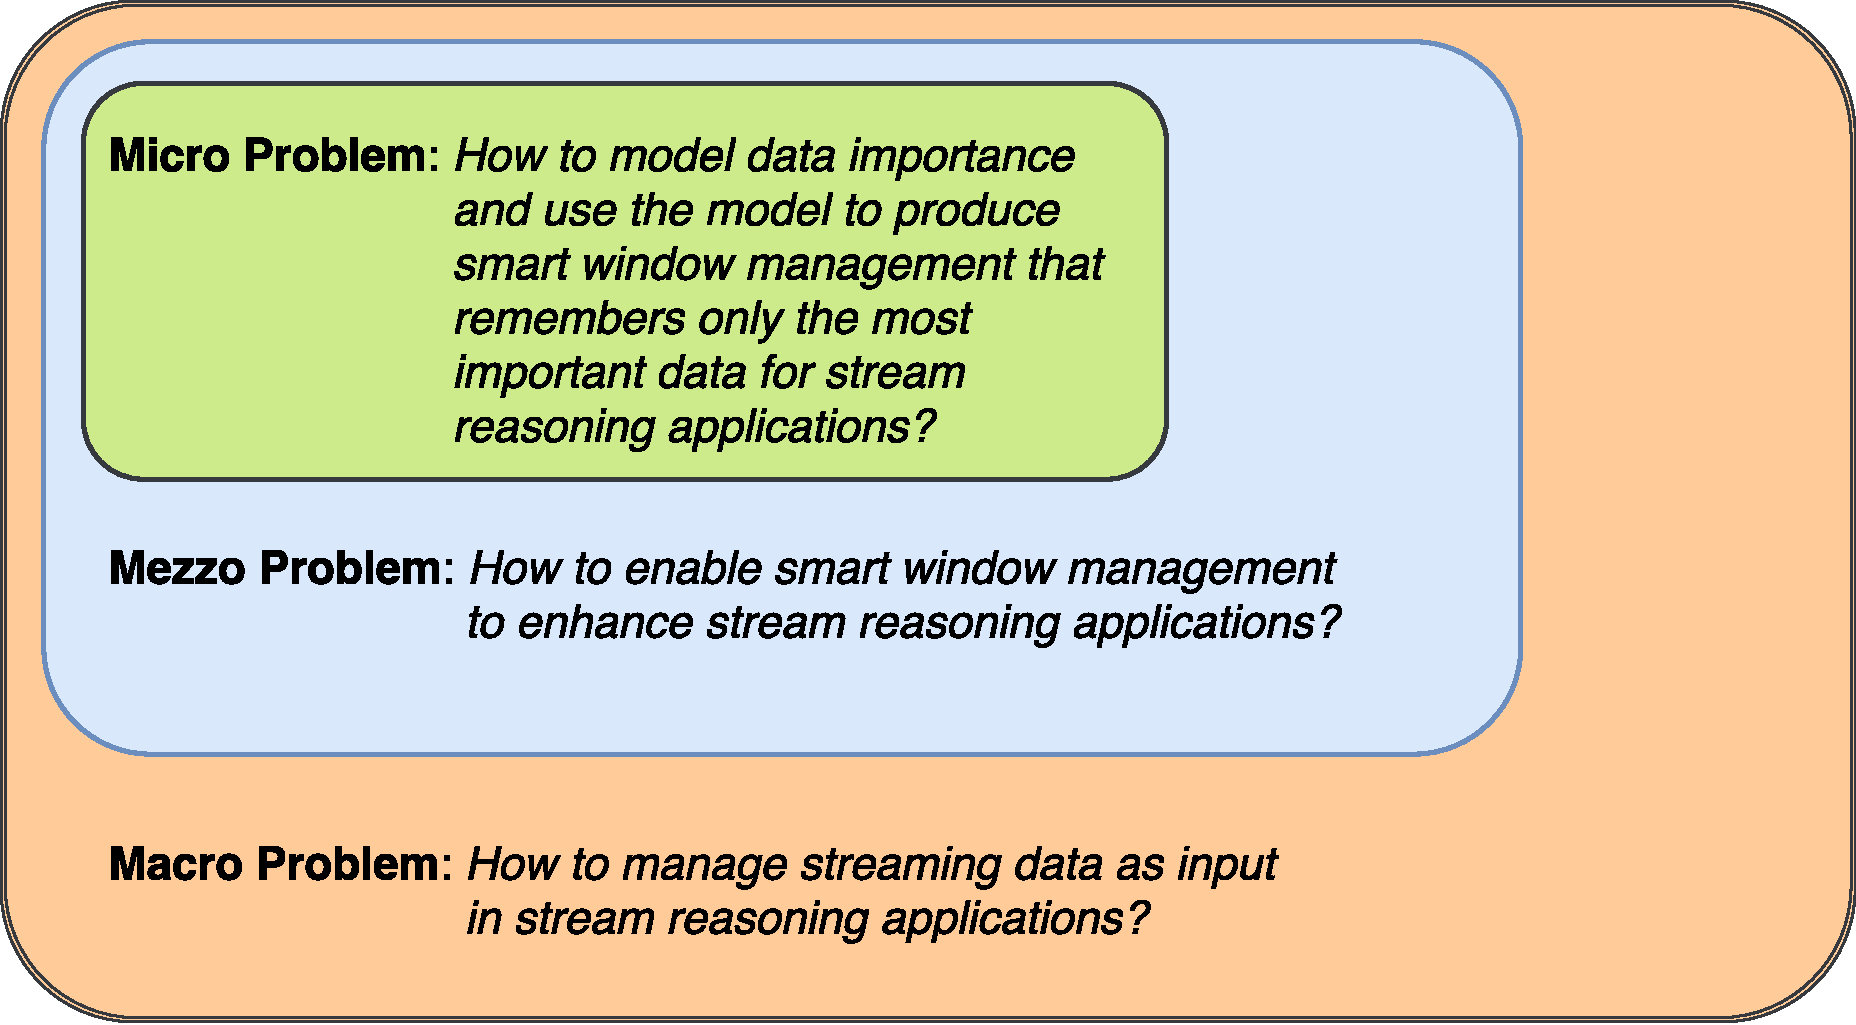
\includegraphics[width=5in]{img/1-rq.pdf}
	\caption{\textbf{Research Questions}}
	\label{fig:1-rq} 
\end{figure}

In general, this dissertation targets on streaming data management for stream reasoning. 
As mentioned in previous sections, the silent temporal assumption and FIFO management strategy are neither adequate to deal with problems of early eviction and early expiration. 
After all, these two problems influence the performance of the stream reasoning systems. 
So, a more concrete question is how to enable windows to manage streaming data in a both smart and efficient way, such that the stream reasoning systems can be enhanced. 
In order to answer this question, this work needs to define what a smart window management refers to, then how to enable this smart management. 
Figure \ref{fig:1-rq} displays the three research questions in a micro-mezzo-macro \cite{lacasse2015making} fashion.

The micro problem itself has defined what a smart window management is: to remember only the most important data. 
In order to enable this smartness, the system has to know what the data importance is about, and how to rank the data based on its importance. 
Thus the problem boils down to model data importance that can be used during window managing streaming data. 

The mezzo problem is a level more general than the micro problem.
What it asks for is that if there is a solution for the micro problem, how to use this solution to enhance stream reasoning applications, and how to prove that this solution is general in a way such that it can be adapted into different scenarios and use cases. 
The window should know which data is more important than others. 
By only keeping the important data, window size can be shrank while the ability to answer the query is not influenced.
Keeping a smaller window size means smaller amount of data, which saves memory and reduces query execution time. 

The macro problem is how to manage the torrent, heterogeneous and large-scale streaming data for processing and reasoning. 
This problem is about the general vision of stream reasoning, including aspects of data model, query model, window operator, data processing etc, thus can be used to provide future research directions of this dissertation.  
%
\section{Dissertation Contributions}

\begin{figure}[!htbp]
	\centering
    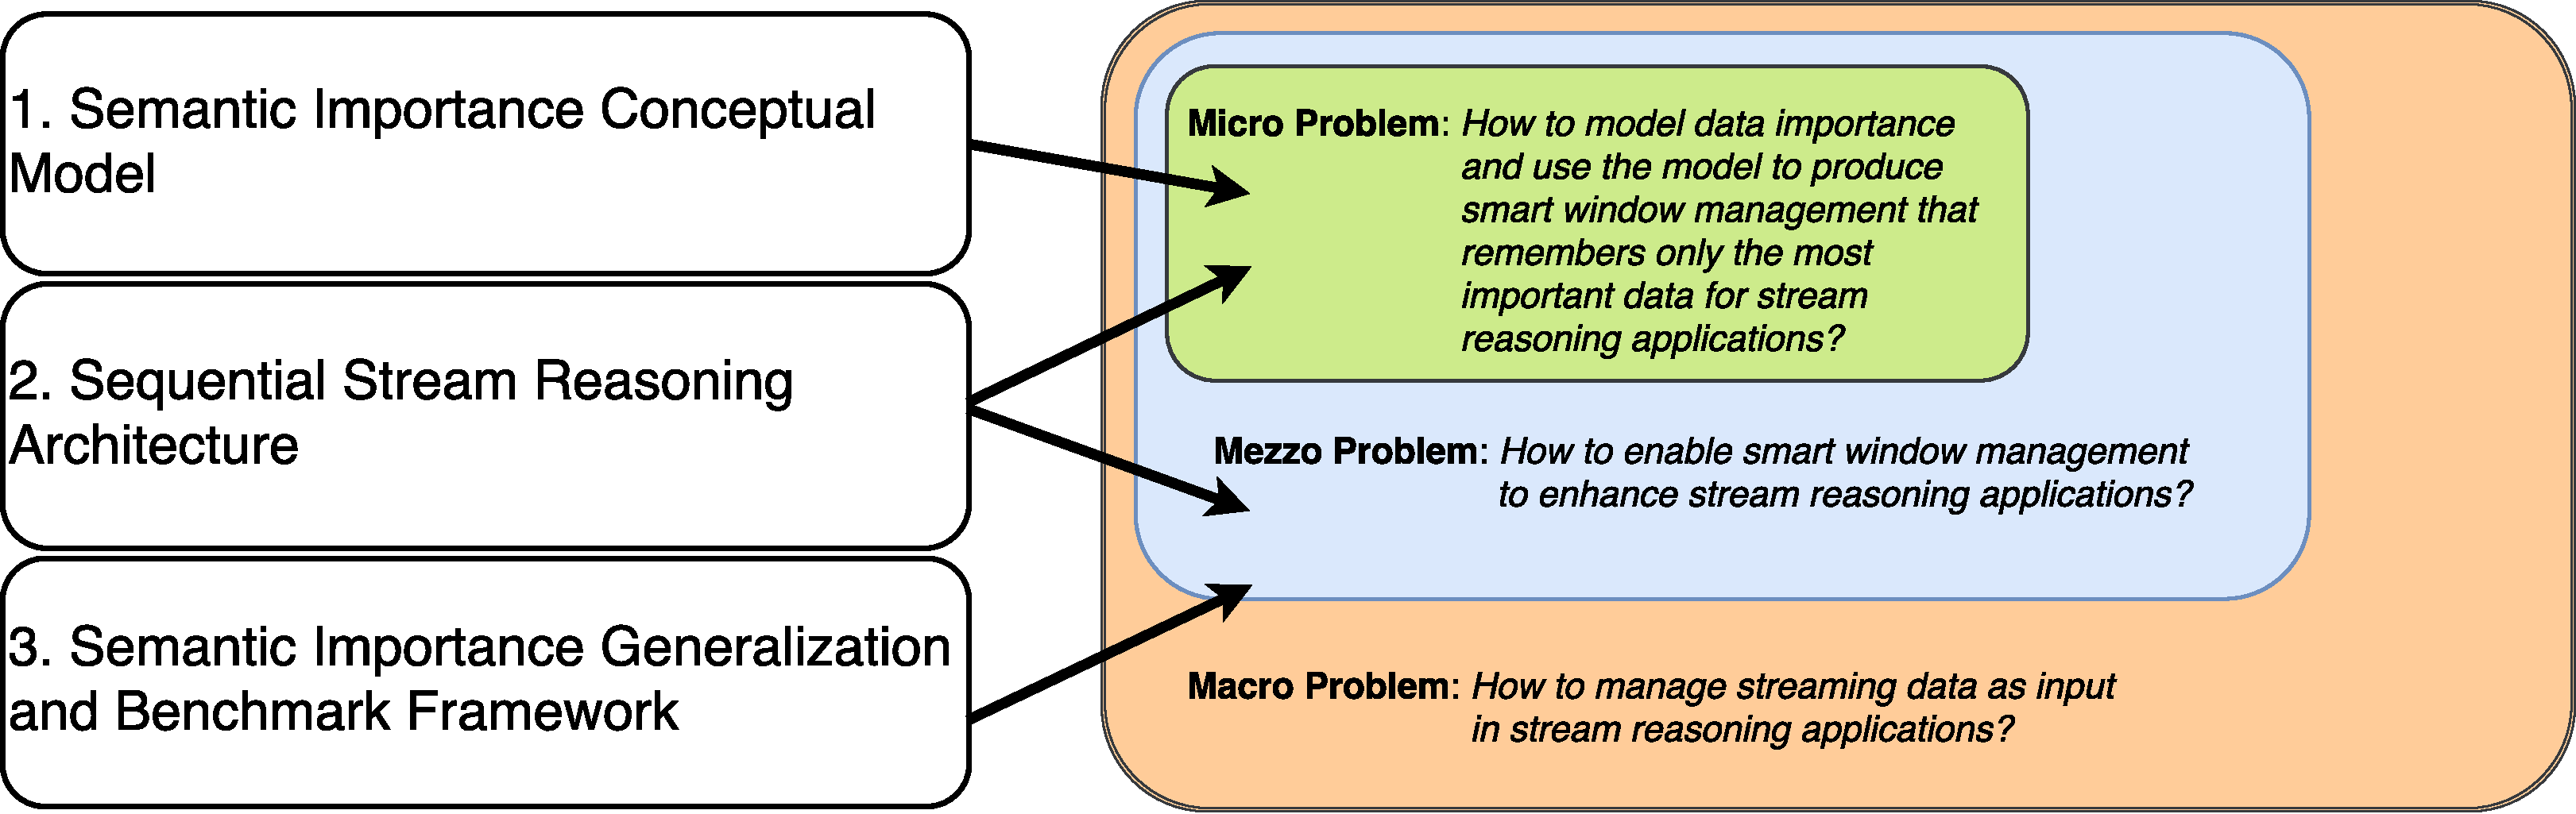
\includegraphics[width=5in]{img/1-dc.pdf}
    \caption{\textbf{Dissertation Contributions}}
    \label{fig:1-dc}
\end{figure}

This dissertation claims three contributions.
Figure \ref{fig:1-dc} shows each of them and how they can be mapped to help answer the research questions.

\textbf{Semantic Importance Conceptual Model}
The notion of ``semantic importance'' is proposed to describe the data importance from various streaming data orderings. 
Semantic importance currently includes four aspects,``provenance'', ``query participation'', ``trustworthiness'', and ``query relevance''.
These four aspects provide a preliminary set of metrics according to which different order-aware window management strategies can be constructed.
Each data item is associated with a semantic importance indicator that is embodied as a mathematical priority vector.
Priority vectors are comparable thus data can be ranked.
With this ranking, more important data can be preserved while less important data will be evicted, no matter how different orderings are chosen as semantic importance to be deployed in the system.

\textbf{Sequential Stream Reasoning Architecture}
Semantic importance is a new concept.
Most existing stream reasoning applications are not compatible with semantic importance.
However, in order to show how to deploy it and how many benefits it can bring, the sequential stream reasoning architecture has been designed and implemented.
This architecture has one window design, and four components arranged in a sequential work-flow: 
(1) a data consumption component that consumes streaming data and sends it to the streaming window;
(2) a query execution component that evaluates a standard SPARQL query against the data in the triplestore and background ontology; 
(3) a result explanation component that uses the query and reasoning process to explain how the result is generated;
(4) a data eviction component that evicts selected data from the window and then returns to the data consumption component for continuous processing.  
All the four sequential components are interacting with the window from time to time.
Leveraging this architecture and semantic importance, two use cases were implemented from different domains. 
The first use case explores soccer offside detection, where query contribution, provenance and query relevance are selected and evaluated. 
The second use case detects data exfiltration event in the insider threat domain, where trustworthiness and provenance are leveraged.
The results have shown that semantic importance is able to improve precision, response time, memory consumption, and throughput for stream reasoning.

\textbf{Semantic Importance Generalization and Benchmark Framework}
In order to provide the empirical support for the generalization of semantic importance, an evaluation framework is designed and implemented.
This framework generalizes semantic importance by connecting it with the state-of-the-art stream reasoning techniques, such as continuous query languages, window semantics, operational semantics etc. 
It also provides a comprehensive benchmark test bed, with various benchmark configuration parameters. 
It can work with either user provided data, or a default data generator that is evolved from LUBM data generator \cite{guo2005lubm}.
In this dissertation, the detailed experimental results are visualized and analyzed to illustrate the superiority of the semantic importance.